\documentclass[size=14pt,
style=paintings
%style=aggie
%style=bframe
%style=ciment
%style=elcolors
%style=fyma blue
%style=fyma brown
%style=fyma gray
%style=fyma green
%style=fyma orange
%style=horatio
%style=husky
%style=ikeda
%style=jefka blue
%style=jefka brown
%style=jefka seagreen
%style=jefka white
%style=klope blackwhite
%style=klope bluewater
%style=klope pastelflower
%style=klope spring
%style=paintings charon
%style=paintings europa
%style=paintings goldengate
%style=paintings holywood
%style=paintings lamentation
%style=paintings maythird
%style=paintings moitessier
%style=paintings pearlearring
%style=paintings skater
%style=paintings syndics
%style=pazik brown
%style=pazik red
%style=sailor chocolate
%style=sailor cocktail
%style=sailor river
%style=sailor sea
%style=sailor wine
%style=simple
]{powerdot}

\pdsetup{palette=Skater}

\usepackage[utf8]{inputenc}
\usepackage{xcolor}
\title{Introdução ao Linux}

\date{Outubro, 2013}

\newenvironment{vslide}{\vspace{\stretch{1}}}{\vspace{\stretch{1}}}

\begin{document}
\maketitle

%%-------------------------------------------------------------------------------------
\begin{slide}{Unix}
\twocolumn{
%\onslide{2-}{}
\vspace{1cm}
Ken Thompson

\vspace{.5cm}
Dennis Ritchie
}
{
   \begin{figure}[!h]
  \includegraphics[scale=0.2]{imagens/att}
   \end{figure}
}

\textbf{Filosofia Unix}:
\begin{itemize}
\item Arquivos de texto armazenam dados.
\item Sistema de arquivos hierárquico.
\item Tratamento de alguns dispositivos como arquivos.
\item Programas pequenos se unem para realizar uma tarefa maior.
\end{itemize}
\end{slide}

\begin{slide}{Tanenbaum e o MINIX}

\begin{vslide}
\textbf{Andrew D. Tanenbaum}, em 1987, escreveu o livro {\color{blue}Operating Systems: Design and Implementation}\\ (``Sistemas Operacionais: Projeto e Implementação'').
\\
\vspace{.5cm}
MINIX foi usado como material de apoio ao livro.

\vspace{0.5cm}
Inspirado no MINIX, \textbf{Linus Torvalds} criou seu próprio sistema operacional, o \textit{kernel} do \textbf{Linux}.
\vspace{0.5cm}
\end{vslide}

\end{slide}

\begin{slide}{Tanenbaum e o MINIX}

\footnotesize \emph{Hello everybody out there using minix -
 I'm doing a (free) operating system (just a hobby, won't be big and professional like gnu) for 386(486) AT clones. This has been brewing since april, and is starting to get ready. I'd like any feedback on things people like/dislike in minix, as my OS resembles it somewhat (same physical layout of the file-system (due to practical reasons) among other things).}

\vspace{0.5cm}
 \emph{I've currently ported bash(1.08) and gcc(1.40), and things seem to work. This implies that I'll get something practical within a few months, and I'd like to know what features most people would want. Any suggestions are welcome, but I won't promise I'll implement them :-)}
\vspace{0.5cm}

 \emph{Linus (torvalds@kruuna.helsinki.fi)
 PS. Yes – it's free of any minix code, and it has a multi-threaded fs. It is NOT portable (uses 386 task switching etc), and it probably never will support anything other than AT-harddisks, as that's all I have :-(.
}
\vspace{0.2cm}

 \emph{— Linus Torvalds}
\end{slide}

\section{Conhecendo o Linux}

\begin{slide}{GNU/Linux}

\begin{vslide}
O Linux que conhecemos na verdade é o \textbf{GNU/Linux}.

\vspace{0.5cm}

A maioria das distribuições utilizam o \textit{kernel} do Linux em conjunto com \textit{softwares} GNU.
\end{vslide}

\end{slide}

\begin{slide}{Projeto GNU}
\begin{vslide}
Iniciado em 1983 por \textbf{Richard Stallman} enquanto trabalhava no laboratório de inteligência artificial no MIT.

\vspace{0.5cm}
\begin{itemize}
\item \textit{Software} livre
\item \textit{Software} proprietário
\end{itemize}

\vspace{0.5cm}
Stallman também criou a ``Free Software Foundation'' que administra as licenças GNU, como a GPL (\textit{General Public License}).
\end{vslide}
\end{slide}

\begin{slide}{Kernel}


   \begin{figure}[!h]
  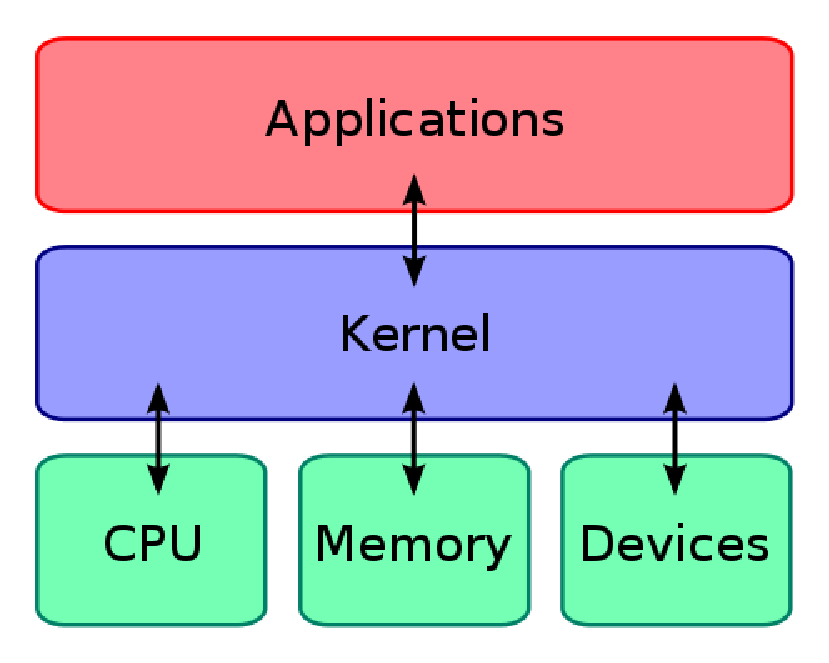
\includegraphics[scale=.8]{imagens/kernel1}
   \end{figure}

\end{slide}

\begin{slide}{Distribuições}
\begin{vslide}
O que se conhece popularmente como Linux, é na verdade apenas o \textit{kernel}, utilizado em todas as distribuições.

\vspace{0.5cm}
Distribuições nada mais são que o \textit{kernel} do Linux juntamente com alguns outros \textit{softwares} (em sua maioria GNU, mas não necessariamente) que dão funcionalidade ao sistema.

   \begin{figure}[!h]
  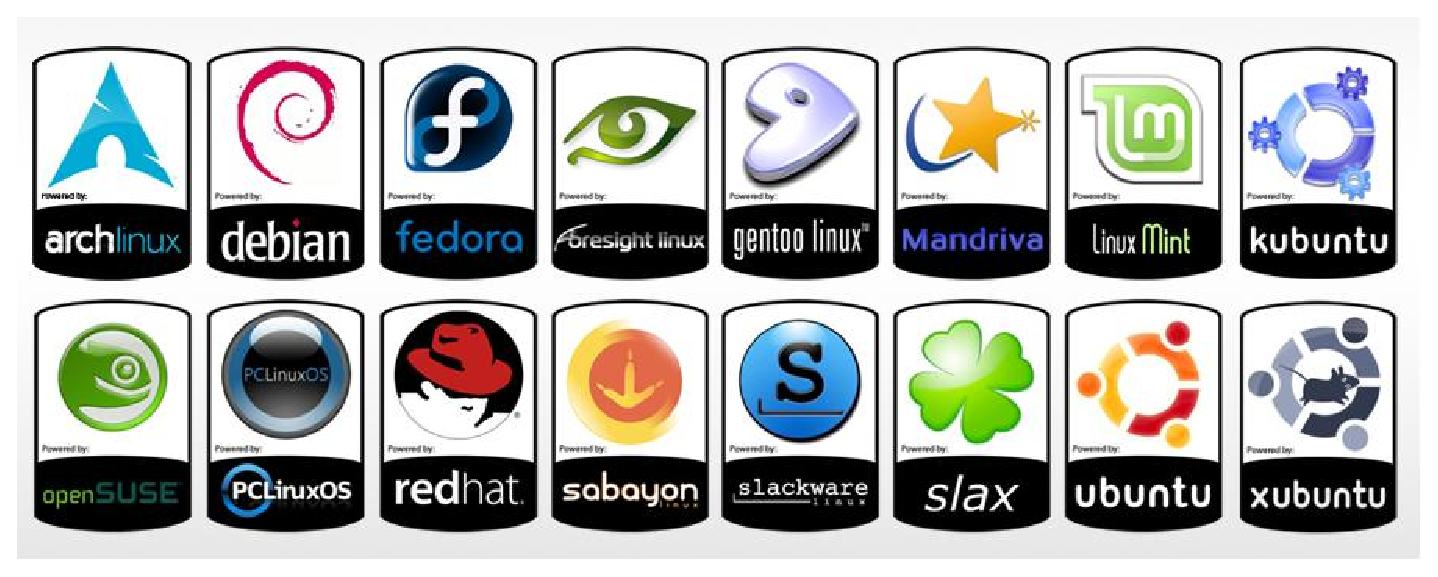
\includegraphics[scale=0.4]{imagens/distro}
   \end{figure}
\end{vslide}
\end{slide}

\begin{slide}{Desktop Environment}
  \centering
   \begin{figure}[!h]
  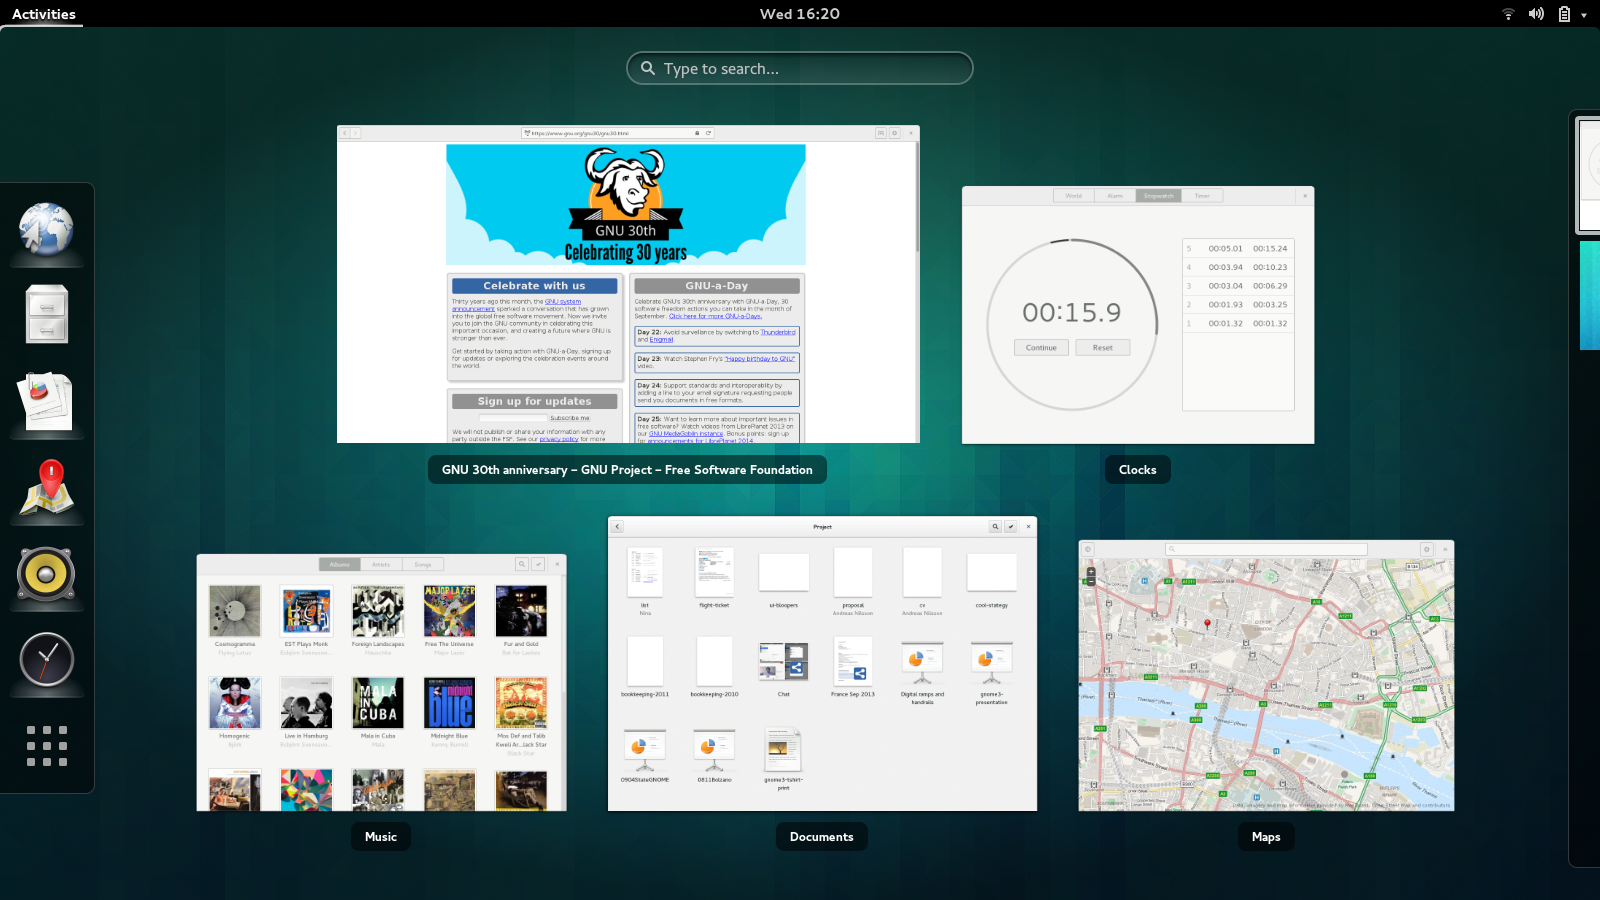
\includegraphics[scale=0.28]{imagens/gnome}
   \end{figure}
\end{slide}

\begin{slide}{Desktop Environment}
  \centering
   \begin{figure}[!h]
  \includegraphics[scale=0.3]{imagens/xfce}
   \end{figure}
\end{slide}

\begin{slide}{Desktop Environment}
  \centering
   \begin{figure}[!h]
  \includegraphics[scale=0.28]{imagens/cinnamon}
   \end{figure}
\end{slide}

\begin{slide}{Window Manager}
\begin{vslide}

Window Manager gerencia funções como:

\begin{itemize}
\item Aparência de janelas.
\item Comportamento na troca de janelas (alt + Tab).
\end{itemize}

\end{vslide}
\end{slide}

\begin{slide}{Alternativas de uso}
\begin{vslide}

\begin{itemize}
\item Máquina Virtual
\item Dual-boot
\item Wine
\end{itemize}

\end{vslide}
\end{slide}

\end{document}